\paragraph{Impact of multi-layer attention}
\label{subsec:exp3}

The fairseq CNN features attention from all layers of the
decoder. Is the possibility to focus on different aspects of the input
while decoding from different layers crucial to the better
generalization skills of the CNN? Fig.~\ref{fig:exp3} reports model
accuracy when using attention only from a subset of the 6
layers. Whereas for the \emph{random} split differences are minimal,
ablating attentions greatly affects the performance on the
compositional splits (although in both cases there is a single ablated
configuration that is as good as the full setup).

\begin{figure}[tb]
    \centering
    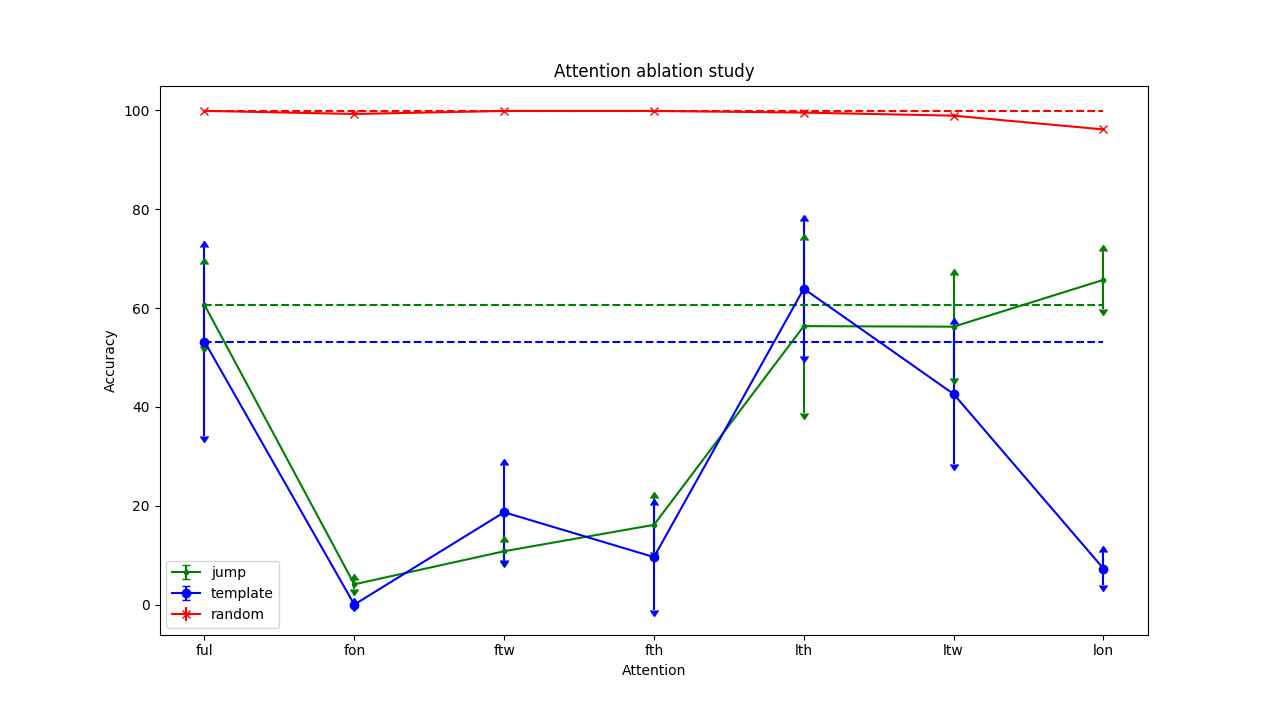
\includegraphics[width=.5\textwidth,keepaspectratio]{figures/attention_exp.png}
    \caption{Accuracy of overall-best model when keeping attention
      only on first layer (\emph{bottom1}), first two layers
      (\emph{bottom2}), \ldots, last two layers (\emph{top2})), top
      layer only (\emph{top1}). Means and standard deviations across 5
      seeds. Dashed lines show full-multi-layer attention results.}
    \label{fig:exp3}
\end{figure}

